\chapter{LİTERATÜR ARAŞTIRMASI}

\lipsum[6]
\parencite{shanvd2005}. 
\lipsum[7] 
\parencite{Zhaopaper}. 
\lipsum[5]
\parencite{he_chen}. 
\lipsum[8]
\acrfull{ldp}, \acrfull{lmp}, \acrfull{lbp} ve \acrfull{hog} çokça kullanılmıştır.

\parencite{barlett} 
\lipsum[10]
\acrfull{svm}  \acrfull{svm} dayalı özellik entegrasyonu ile birleştirerek bir yöntem sundular . 
%(Mohammad ve Ali, 2011),
\parencite{mohammad} çalışmalarında, \acrshort{lmp} yöntemini kullanmışlardır
% (Shan vd., 2009)
\parencite{SHAN2009}   \acrshort{lbp}  \acrshort{svm} 

\lipsum[11]


% (Zhao ve Zhang, 2011)
\parencite{zhaoandother}, Pellentesque habitant morbi tristique senectus et netus et malesuada fames ac turpis egestas.
%(Akyol ve Şahin, 2016),
\parencite{akyol} Donec odio elit, dictum in, hendrerit sit amet, egestas sed, leo. Praesent feugiat
sapien aliquet odio. Integer vitae justo
% (Gacav vd., 2018)
\parencite{gacav2018} Integer vitae justo. Aliquam vestibulum fringilla lorem. Sed neque
lectus, consectetuer at.
% (He ve Chen, 2020) 
\parencite{he_chen} Proin eu metus. Sed porttitor. In hac habitasse platea dictumst. Suspendisse eu
lectus.
% (Özbey ve Topal, 2018)
\parencite{ozbey2018}, Suspendisse vel felis. Ut lorem lorem, interdum eu, tincidunt sit amet, laoreet vitae, arcu. Aenean faucibus pede eu ante
% (Akcakoca ve Gökmen, 2015)
\parencite{akcakoca}, Quisque vehicula, urna sed ultricies auctor, pede lorem egestas dui, et convallis
elit erat sed nulla.
%(Bayrakdar vd., 2016)
\parencite{bayrakdar2017} Fusce mauris. Vestibulum luctus nibh at lectus. Sed bibendum, nulla a faucibus
semper, leo velit ultricies tellus 

Vivamus viverra fermentum felis. Donec nonummy pellentesque ante. Phasellus
adipiscing semper eli
%(Soyel ve Demirel, 2008)
\parencite{soyeldemirel} Nulla ac nisl. Nullam urna nulla, ullamcorper in, interdum sit amet, gravida ut, risus. Aenean ac enim \%88.5 Nullam urna.
\parencite{Ghimire_2013} vivamus viverra fermentum felis. Donec nonummy pellentesque ante. Phasellus
adipiscing semper elir.  

%(Gacav vd., 2016)
\parencite{gacav2016} Nulla ac nisl. Nullam urna nulla, ullamcorper in, interdum sit amet, gravida ut, risus. Aenean ac enim \%88.5 Nullam urna.
2017 yılında \parencite{Gacav2017} Nulla ac nisl. Nullam urna nulla, ullamcorper in, interdum sit amet, gravida ut, risus. Aenean ac enim \%88.5 Nullam urna.
\parencite{aksoy2016} Quisque vehicula, urna sed ultricies auctor, pede lorem egestas dui, et convallis
 \acrfull{dke} elit erat sed nulla. \acrshort{dke} Sed feugiat. Cum sociis natoque penatibus et magnis dis parturient montes, nascetur
ridiculus mus.
 
\acrfull{cnnetwork}, yüz ifadesi tanıma için kullanılan bir başka popüler yöntemdir ve geleneksel öznitelik çıkartma yöntemlerine kıyasla bu alandaki çalışmalarda kulanımı giderek artmaktadır. 
%(Tümen vd.,2017) 
\parencite{tumen2017}  Ut lectus eros, malesuada sit amet, fermentum eu, sodales cursus, magna \acrshort{cnnetwork}  \%57.1 Aenean faucibus pede eu ante.

% (Li vd.,2017) 
\parencite{li2017}  Integer arcu est, nonummy in, fermentum faucibus.
% (Abanoz ve Çataltepe, 2018)
\parencite{abanoz2018} Mauris felis odio.

% (Akay ve Arıca, 2018) 
\parencite{akayarıca2018} Suspendisse vel felis. Ut lorem lorem, interdum eu, tincidunt sit amet, laoreet vitae,arcu.
% (Liu vd.,2020) (Feng ve Shao, 2020)
\parencite{liu2020}, Donec pellentesque, erat ac sagittis semper, nunc dui lobortis purus, quis
congue purus metus ultricies tellus \acrshort{svm}, \parencite{fengshao2020} , Proin et quam. Class aptent taciti sociosqu. 
% (Videla ve Kumar, 2020)
\parencite{videlakumar2020} nubia nostra, per inceptos hymenaeos.
% (Mohan vd. 2020)
\parencite{mohan2021} Class aptent taciti sociosqu ad litora torquent per conubia nostra, per inceptos hymenaeos.



% Basit iki terimle \acrfull{OBEB} ve \acrfull{OKEK} kısaltmaları anlatabiliriz. İster kısaltmasını \acrshort{OBEB}, isterseniz de uzun açılımını \acrlong{OKEK} yazdırabilirsiniz. Bunu yapabilmek için dosyanın başında terimleri tanımlamanız gereklidir. İsterseniz matematik terimlerini de, örneğin \acrshort{pi} böyle tanımlayabilirsiniz. Uzun uzun \acrfull{pi} yazmanız gerekmez. 

% Teorem yazmak isterseniz:
% \begin{theorem}[Öklid]
%  İki noktadan bir ve yalnız bir doğru geçer.
% \end{theorem}

% İspat yazmak isterseniz:
% \begin{ispat}[Tezin en önemli ispatı]
% x=10
% \end{ispat}
% \lipsum[1-2]
% \begin{figure}[h]
% \centering
% 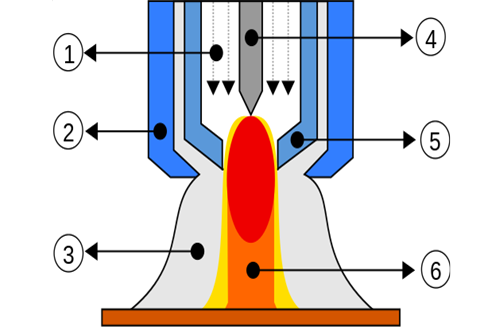
\includegraphics[width=\textwidth]{gorseller/ptaTorc}
% \caption{PTA Torç}\label{fig:PtaTorc1}
% \end{figure}
% \lipsum[1-2]
% \begin{table}
% \centering
% \caption{Deneme Tablosu.}\label{tab:den1}
% \begin{tabular}{|l|l|l|}
% \hline
% sıra   & sayı   & toplam \\ \hline
% 1      & 2      & 3      \\ \hline
% Kelime & deneme & son    \\ \hline
% \end{tabular}
% \end{table}


% % \section{Literatür Araştırması Birinci Derece Başlık}
% % \lipsum[1-2]
% \begin{figure}[h]
% \centering
% 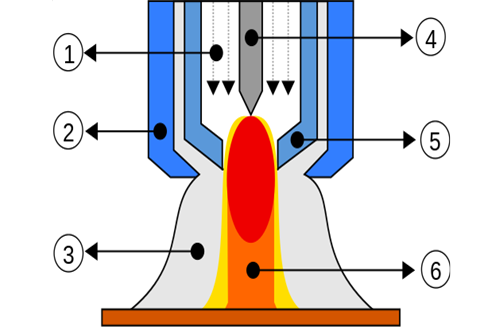
\includegraphics[width=\textwidth]{gorseller/ptaTorc}
% \caption{PTA Torç}\label{fig:PtaTorc1}
% \end{figure}
% \lipsum[1-2]
% \begin{table}
% \centering
% \caption{Deneme Tablosu.}\label{tab:den1}
% \begin{tabular}{|l|l|l|}
% \hline
% sıra   & sayı   & toplam \\ \hline
% 1      & 2      & 3      \\ \hline
% Kelime & deneme & son    \\ \hline
% \end{tabular}
% \end{table}
% Teorem yazmak isterseniz:
% \begin{theorem}[Öklid]
%  İki noktadan bir ve yalnız bir doğru geçer.
% \end{theorem}

% İspat yazmak isterseniz:
% \begin{ispat}[Tezin en önemli ispatı]
% x=10
% \end{ispat}

% % \subsection{Literatür Araştırması ikinci derece başlık}
% % \lipsum[1-2]
% \begin{figure}[h]
% \centering
% 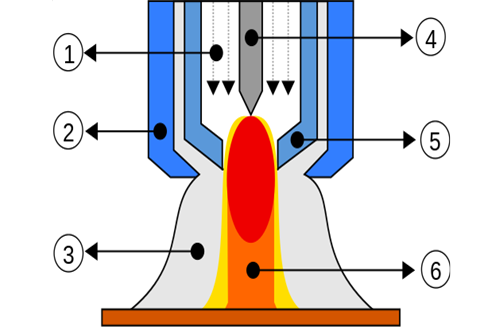
\includegraphics[width=\textwidth]{gorseller/ptaTorc}
% \caption{PTA Torç}\label{fig:PtaTorc1}
% \end{figure}
% \lipsum[1-2]
% \begin{table}
% \centering
% \caption{Deneme Tablosu.}\label{tab:den1}
% \begin{tabular}{|l|l|l|}
% \hline
% sıra   & sayı   & toplam \\ \hline
% 1      & 2      & 3      \\ \hline
% Kelime & deneme & son    \\ \hline
% \end{tabular}
% \end{table}

% Teorem yazmak isterseniz:
% \begin{theorem}[Öklid]
%  İki noktadan bir ve yalnız bir doğru geçer.
% \end{theorem}

% İspat yazmak isterseniz:
% \begin{ispat}[Tezin en önemli ispatı]
% x=10
% \end{ispat}

% % \subsubsection{Literatür araştırması dördüncü derece başlık}
% \lipsum[1-2]
% \begin{figure}[h]
% \centering
% 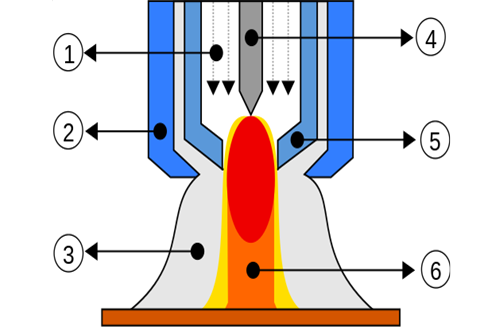
\includegraphics[width=\textwidth]{gorseller/ptaTorc}
% \caption{PTA Torç}\label{fig:PtaTorc1}
% \end{figure}
% \lipsum[1-2]
% \begin{table}
% \centering
% \caption{Deneme Tablosu.}\label{tab:den1}
% \begin{tabular}{|l|l|l|}
% \hline
% sıra   & sayı   & toplam \\ \hline
% 1      & 2      & 3      \\ \hline
% Kelime & deneme & son    \\ \hline
% \end{tabular}
% \end{table}

% Teorem yazmak isterseniz:
% \begin{theorem}[Öklid]
%  İki noktadan bir ve yalnız bir doğru geçer.
% \end{theorem}

% İspat yazmak isterseniz:
% \begin{ispat}[Tezin en önemli ispatı]
% x=10
% \end{ispat}